\documentclass[conference]{IEEEtran}
\usepackage[utf8]{inputenc}
\usepackage{kotex}
\usepackage{newtxtext,newtxmath}
\usepackage{cite}
\usepackage{amsmath,amssymb,amsfonts}
\usepackage{graphicx}
\usepackage{booktabs}
\usepackage{hyperref}

\graphicspath{{../../../submission/data/analysis/figures/}}

\begin{document}

\sloppy
\setlength{\parskip}{0.3em}
\setlength{\parindent}{1em}

\renewcommand{\thesubsection}{\arabic{subsection}}

\title{LLMDump: LLM-Powered Zero-Day Vulnerability Prediction for AI Systems}

\author{\IEEEauthorblockN{Susie Choi}
\IEEEauthorblockA{GitHub: \url{https://github.com/susie-Choi/llmdump}\\
Email: sschoidev@gmail.com}}

\maketitle

\pagestyle{plain}
\thispagestyle{plain}

\begin{abstract}
2022년 11월 ChatGPT 출시 이후 AI 관련 CVE가 폭발적으로 증가하고 있다(2023년 54개 → 2025년 241개, +346\%). 그러나 기존 취약점 탐지 도구들은 CVE 발표 이후에만 작동하는 사후 대응 방식이다. 본 연구는 CVE 발표 전 단계에서 AI 관련 취약점을 예측하는 LLMDump 시스템을 개발하고 있다. LLMDump는 GitHub API 기반 개발 신호 수집, Neo4j 그래프 데이터베이스를 활용한 취약점 패턴 학습, LLM 기반 RAG(Retrieval-Augmented Generation)를 통한 위험도 예측을 통합한다. 현재까지 10년간(2015-2025) 255,923개 CVE를 분석하고, AI 관련 CVE 462개를 식별했다. AI 관련 CVE의 58.2\%가 HIGH 이상의 심각도를 보여 높은 위험성을 나타냈으며, Prompt Injection(16.0\%), ML 플랫폼 취약점(32.5\%) 등 새로운 공격 벡터가 부상하고 있다. 향후 GitHub 개발 신호 분석과 LLM 기반 예측을 통해 AI 시스템의 zero-day 취약점을 사전에 탐지하는 시스템으로 발전시킬 계획이다.
\end{abstract}

\section{서론}

현대 소프트웨어 개발은 오픈소스 생태계에 크게 의존하고 있으며, 2022년 11월 ChatGPT 출시 이후 AI/ML 라이브러리의 사용이 폭발적으로 증가했다. LangChain, Hugging Face, PyTorch, Gradio 등 AI 프레임워크와 플랫폼이 빠르게 확산되면서, 이들의 보안 취약점도 급증하고 있다.

본 연구에서 수집한 데이터에 따르면, AI 관련 CVE는 2023년 54개에서 2024년 167개(+209.3\%), 2025년 241개(+44.3\%)로 폭발적으로 증가했다. 특히 AI 관련 CVE의 58.2\%가 HIGH 이상의 심각도를 보여, 일반 소프트웨어 취약점보다 높은 위험성을 나타낸다.

더욱 심각한 문제는 취약점이 CVE로 등록되기 전 이미 공격자들이 악용하고 있다는 점이다. AI 시스템은 Prompt Injection, Data Poisoning, Adversarial Attack 등 전통적인 보안 도구로는 탐지하기 어려운 새로운 공격 벡터에 노출되어 있다. OWASP LLM Top 10 (2023)은 이러한 위협을 체계화했으나, 실제 CVE 발표 전 단계에서 이를 탐지하는 연구는 부족한 실정이다.

오픈소스 보안을 위해 사용되는 기존 도구들은 근본적인 한계를 가진다. GitHub Dependabot, Snyk 등 CVE 기반 도구는 이미 알려진 CVE 데이터베이스를 기반으로 작동하여, 취약점이 공개된 후에야 대응이 시작된다. EPSS(Exploit Prediction Scoring System)도 CVE 발표 이후에만 점수가 부여된다. 정적 분석 도구는 개별 코드의 구조적 취약점을 찾을 수 있지만, AI 시스템 특유의 공격 패턴(Prompt Injection 등)을 탐지하지 못한다.

본 연구에서는 이러한 한계를 극복하기 위해 다음과 같은 연구 질문을 설정한다:

\noindent\textbf{RQ1 (Early Detection)}: GitHub 개발 신호(Commit, PR, Issue) 분석이 CVE 발표 전 단계에서 AI 관련 취약점을 조기에 탐지할 수 있는가?

\noindent\textbf{RQ2 (Pattern Learning)}: RAG 기반 LLM 분석이 과거 AI 관련 CVE 패턴을 학습하여, 새로운 취약점 도입을 예측할 수 있는가?

\noindent\textbf{RQ3 (AI-Specific Threats)}: Prompt Injection, Data Poisoning 등 AI 특화 공격 패턴을 기존 방법론보다 효과적으로 탐지할 수 있는가?

본 연구의 목적은 CVE 발표 이전 단계에서 AI 관련 취약점을 예측하는 시스템을 구축하는 것이다. 핵심 아이디어는 단순히 개별 코드의 취약점을 찾는 것이 아니라, AI/ML 생태계의 개발 신호를 분석하여 과거 취약점 패턴과의 유사도를 측정하는 것이다.


\section{배경: AI 관련 CVE 현황}

\subsection{10년간 CVE 추이 (2015-2025)}

NVD API 2.0을 통해 2015-2025년 CVE 데이터를 수집했다. 표 \ref{tab:cve_10year}는 10년간 CVE 발표 현황을 보여준다.

\begin{table}[h]
\centering
\caption{연도별 CVE 발표 현황 (2015-2025)}
\label{tab:cve_10year}
\begin{tabular}{rrr}
\toprule
\textbf{연도} & \textbf{CVE 수} & \textbf{전년 대비} \\
\midrule
2015 & 6,595 & - \\
2016 & 6,517 & -1.2\% \\
2017 & 18,113 & +178.0\% \\
2018 & 18,154 & +0.2\% \\
2019 & 18,938 & +4.3\% \\
2020 & 19,222 & +1.5\% \\
2021 & 21,950 & +14.2\% \\
2022 & 26,431 & +20.4\% \\
2023 & 30,949 & +17.1\% \\
2024 & 40,704 & +31.5\% \\
2025 & 48,350 & +18.8\% \\
\midrule
\textbf{합계} & \textbf{255,923} & \\
\bottomrule
\end{tabular}
\end{table}

\begin{figure}[h]
\centering
\includegraphics[width=0.48\textwidth]{fig1_cve_trend_10year.jpg}
\caption{10년간 CVE 발표 추이 (2015-2025). 2023년 이후(Post-ChatGPT)가 강조됨.}
\label{fig:cve_trend}
\end{figure}

전체 CVE는 2015년 6,595개에서 2025년 48,350개로 약 7.3배 증가했다. 특히 2024년(+31.5\%)과 2025년(+18.8\%)의 급격한 증가가 주목된다.

\subsection{AI 관련 CVE 분석 (2023-2025)}

OWASP LLM Top 10을 기반으로 14개 키워드를 정의하여 AI 관련 CVE를 식별했다: prompt injection, jailbreak, data poisoning, adversarial, langchain, llama, ollama, openai, chatgpt, large language model, huggingface, pytorch, mlflow, gradio.

\begin{figure}[h]
\centering
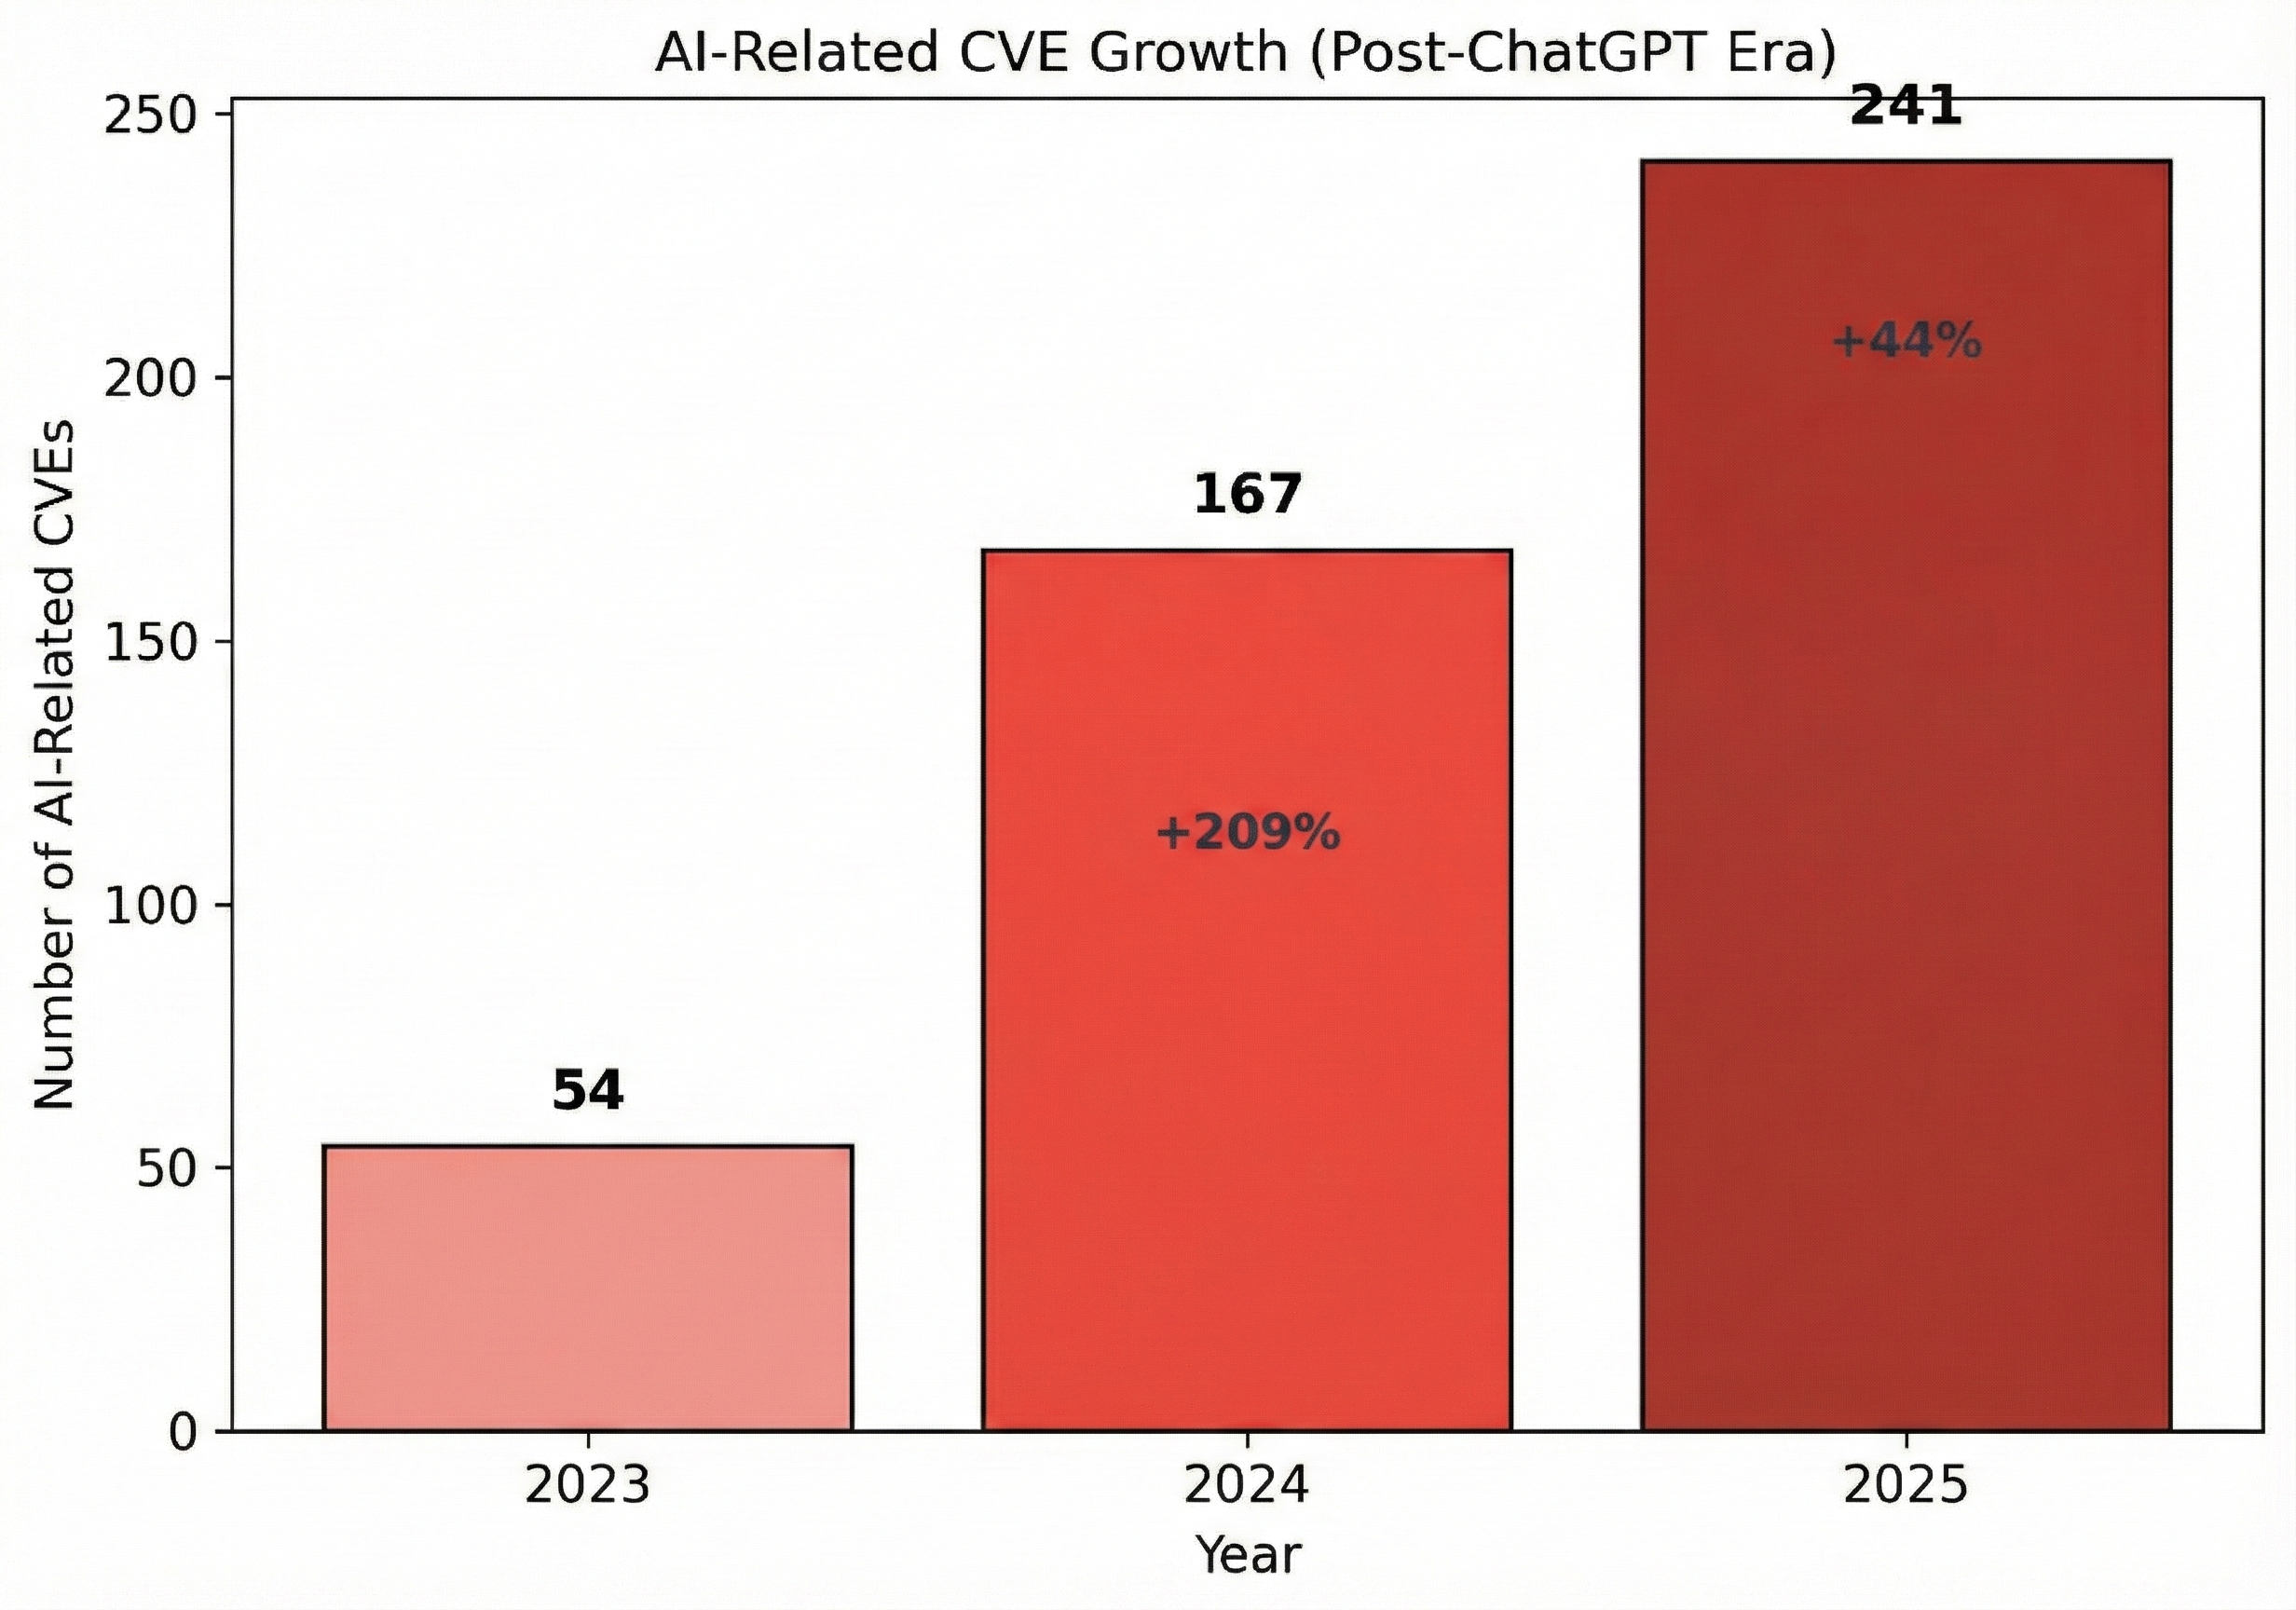
\includegraphics[width=0.4\textwidth]{fig2_ai_cve_growth.jpg}
\caption{AI 관련 CVE 연도별 증가 추이 (2023-2025)}
\label{fig:ai_growth}
\end{figure}

표 \ref{tab:ai_cve}는 AI 관련 CVE의 연도별 현황을 보여준다.

\begin{table}[h]
\centering
\caption{AI 관련 CVE 연도별 현황}
\label{tab:ai_cve}
\begin{tabular}{rrrr}
\toprule
\textbf{연도} & \textbf{AI CVE} & \textbf{성장률} & \textbf{전체 대비} \\
\midrule
2023 & 54 & - & 0.17\% \\
2024 & 167 & +209.3\% & 0.41\% \\
2025 & 241 & +44.3\% & 0.50\% \\
\midrule
\textbf{합계} & \textbf{462} & & \textbf{0.38\%} \\
\bottomrule
\end{tabular}
\end{table}

\subsection{심각도 및 카테고리 분석}

표 \ref{tab:severity}는 AI 관련 CVE의 심각도 분포를 보여준다.

\begin{table}[h]
\centering
\caption{AI 관련 CVE 심각도 분포}
\label{tab:severity}
\begin{tabular}{lrr}
\toprule
\textbf{심각도} & \textbf{CVE 수} & \textbf{비율} \\
\midrule
CRITICAL & 80 & 17.3\% \\
HIGH & 189 & 40.9\% \\
MEDIUM & 145 & 31.4\% \\
LOW & 28 & 6.1\% \\
UNKNOWN & 20 & 4.3\% \\
\midrule
\textbf{HIGH 이상} & \textbf{269} & \textbf{58.2\%} \\
\bottomrule
\end{tabular}
\end{table}

\begin{figure}[h]
\centering
\includegraphics[width=0.35\textwidth]{fig3_ai_severity_dist.jpg}
\caption{AI 관련 CVE 심각도 분포}
\label{fig:severity}
\end{figure}

AI 관련 CVE의 58.2\%가 HIGH 이상의 심각도를 보였다(CRITICAL 17.3\%, HIGH 40.9\%). 이는 AI 시스템 취약점이 심각한 보안 위협이 될 수 있음을 나타낸다.

표 \ref{tab:category}는 AI 관련 CVE의 카테고리별 분포를 보여준다.

\begin{table}[h]
\centering
\caption{AI 관련 CVE 카테고리별 분포}
\label{tab:category}
\begin{tabular}{llrr}
\toprule
\textbf{카테고리} & \textbf{설명} & \textbf{CVE 수} & \textbf{비율} \\
\midrule
platform\_ml & ML 플랫폼 & 150 & 32.5\% \\
service\_ai & AI 서비스 & 130 & 28.1\% \\
framework\_llm & LLM 프레임워크 & 87 & 18.8\% \\
attack\_prompt & Prompt Injection & 74 & 16.0\% \\
attack\_poisoning & Data Poisoning & 17 & 3.7\% \\
attack\_adversarial & Adversarial Attack & 4 & 0.9\% \\
\bottomrule
\end{tabular}
\end{table}

\begin{figure}[h]
\centering
\includegraphics[width=0.45\textwidth]{fig4_ai_categories.jpg}
\caption{AI 관련 CVE 카테고리별 분포}
\label{fig:categories}
\end{figure}

카테고리별로는 ML 플랫폼(32.5\%), AI 서비스(28.1\%), LLM 프레임워크(18.8\%), Prompt Injection(16.0\%) 순으로 분포했다. Prompt Injection은 OWASP LLM Top 10의 1위 위협으로, 실제 CVE로 나타나고 있음을 확인했다.


\section{선행 연구}

\subsection{LLM 기반 취약점 탐지}

취약점 탐지 연구는 LLM의 발전과 함께 새로운 국면을 맞이하고 있다. Du et al. (2024)는 Vul-RAG를 제안하여 RAG 기반 LLM으로 취약점을 탐지했다 \cite{vulrag2024}. 그러나 LLM이 취약한 코드와 패치된 코드를 구분하는 정확도는 6-14\%에 불과했으며, Knowledge-level RAG를 통해 16-24\% 향상을 달성했다. Sun et al. (2024)은 GPT-4와 Claude를 활용한 LLM4Vuln 프레임워크를 제안하여 14개의 zero-day 취약점을 발견했다 \cite{sun2024}.

Ma et al. (2024)는 iAudit을 제안하여 Two-stage 접근법(Detector → Reasoner)을 사용했다 \cite{iaudit2025}. GPT-4도 30\% precision에 그쳤으나, fine-tuning과 LLM Agent 조합으로 F1 91.21\%를 달성했다. Ding et al. (2024)는 ``To Err is Machine''에서 16개 LLM을 평가한 결과, SOTA 모델도 54.5\% balanced accuracy에 그쳤으며, 코드 의미론 이해가 핵심 한계임을 밝혔다 \cite{toerr2024}.

\subsection{LLM의 코드 이해 한계}

Jain et al. (2025)는 CoCoNUT 벤치마크를 통해 LLM의 코드 실행 흐름 추적 능력을 평가했다 \cite{coconut2025}. Gemini조차 HumanEval 태스크의 47\%만 정확히 추적했으며, 재귀와 병렬 처리에서는 5\% 미만의 정확도를 보였다. 이는 LLM이 코드의 구조적 패턴은 인식하지만, 실행 의미론 이해에는 한계가 있음을 시사한다.

\subsection{그래프 기반 접근}

Pelofske et al. (2023)은 Neo4j 그래프 데이터베이스를 활용하여 위협 분석을 수행했다 \cite{pelofske2023}. Ohm et al. (2020)은 npm 생태계의 의존성 네트워크를 분석하여 취약점 전파 경로를 연구했다 \cite{ohm2020}. 그러나 이들의 연구는 이미 알려진 CVE의 영향 범위 분석에 한정되었다.

\subsection{AI 시스템 보안}

OWASP LLM Top 10 (2023)은 LLM 애플리케이션의 주요 보안 위협을 정의했다 \cite{owasp2023}. Chen et al. (2025)는 CrAIBench를 통해 AI Agent의 보안 취약점을 평가했으며, memory injection이 prompt injection보다 더 위험함을 밝혔다 \cite{craibench2025}.

\subsection{기존 연구의 한계}

기존 연구들의 한계를 종합하면: (1) CVE 발표 후 사후 분석에 집중, (2) 단일 모델의 낮은 정확도 (6-54\%), (3) AI 특화 공격 패턴 미고려, (4) 개발 과정의 동적 신호 간과. 본 연구는 Multi-Agent 앙상블 접근법을 통해 이러한 한계를 극복하고자 한다.


\section{시스템 아키텍처}

LLMDump 시스템은 바퀴(Wheel) 은유를 사용하여 설계되었다.

\subsection{Spokes (데이터 수집 계층)}

다양한 소스에서 원시 데이터를 수집한다:
\begin{itemize}
\item \texttt{CVECollector}: NVD에서 CVE 데이터 수집 (현재 255,923개)
\item \texttt{GitHubSignalsCollector}: GitHub에서 Commit, PR, Issue 수집
\item \texttt{EPSSCollector}: FIRST에서 악용 가능성 점수 수집
\item \texttt{KEVCollector}: CISA에서 실제 악용 확인 취약점 수집
\end{itemize}

\subsection{Hub (지식 그래프 계층)}

Neo4j 그래프 데이터베이스를 사용하여 데이터를 통합한다. CVE를 중심으로 CWE, EPSS, KEV, Commit과의 관계를 모델링하며, AI 관련 CVE 462개와 관련 패턴을 저장한다.

\subsection{Oracle (예측 엔진)}

LLM 기반 취약점 위험 예측을 수행한다:

\subsubsection{Commit Analyzer}
개별 Commit의 취약점 위험을 분석한다. AI 특화 패턴으로 \texttt{eval()}, \texttt{exec()}, \texttt{pickle.loads()}, unsafe deserialization, prompt template injection 등을 탐지한다.

\subsubsection{Project Oracle}
프로젝트 전체의 취약점 위험을 분석한다. GitHub 활동, Commit 빈도, 보안 관련 Issue/PR, 이전 CVE 패턴(RAG 사용)을 입력으로 사용한다.

RAG 컨텍스트는 다음을 포함한다:
\begin{itemize}
\item 유사 AI 관련 CVE 검색 (OWASP LLM Top 10 기반)
\item 패키지 취약점 히스토리
\item Prompt Injection, Data Poisoning 패턴
\end{itemize}

\subsection{Axle (평가 계층)}

예측 시스템의 성능을 평가한다. 시간 순서를 고려한 검증 방식을 사용하여, 과거 데이터로 학습한 모델이 미래 CVE를 얼마나 정확히 예측하는지 측정한다.


\section{연구 방법}

\subsection{데이터 수집}

NVD API 2.0을 통해 2015-2025년 CVE 데이터를 수집했다. API rate limit(HTTP 429)을 처리하기 위해 분기별 쿼리와 재시도 로직을 구현했다.

AI 관련 CVE 식별을 위해 OWASP LLM Top 10을 기반으로 14개 키워드를 정의했다 (표 \ref{tab:keywords}).

\begin{table}[h]
\centering
\caption{AI 관련 CVE 식별 키워드}
\label{tab:keywords}
\begin{tabular}{ll}
\toprule
\textbf{카테고리} & \textbf{키워드} \\
\midrule
Attack (Prompt) & prompt injection, jailbreak \\
Attack (Poisoning) & data poisoning \\
Attack (Adversarial) & adversarial \\
LLM Framework & langchain, llama, ollama \\
AI Service & openai, chatgpt, large language model \\
ML Platform & huggingface, pytorch, mlflow, gradio \\
\bottomrule
\end{tabular}
\end{table}

\subsection{예측 방법론}

본 연구는 세 가지 분석 방법을 활용한다:

\textbf{키워드 기반 분석}: 25개 보안 관련 키워드와 AI 특화 키워드를 사용하여 Commit Message를 분석한다.

\textbf{LLM 기반 위험도 평가}: Google Gemini 2.5 Flash를 사용하여 코드의 취약점을 분석한다. 프롬프트는 부록 \ref{appendix:prompt}에 제시되어 있다. 입력으로 파일명, Commit SHA, Commit 메시지, 소스 코드를 제공하고, 출력으로 취약점 존재 여부, 발견 사항(유형, 심각도, 위치, 설명, CWE), 신뢰도를 JSON 형식으로 받는다.

\textbf{그래프 기반 RAG}: Neo4j에 저장된 AI 관련 CVE 패턴을 활용하여 유사 취약점을 검색하고 LLM 컨텍스트로 제공한다.

\subsection{실험 설정}

Multi-Agent 앙상블 접근법의 효과를 검증하기 위해 CVE-2025-5120 (CVSS 10.0, Sandbox Escape)이 발생한 huggingface/smolagents 프로젝트를 대상으로 실험을 수행했다.

\textbf{데이터 수집}: GitHub API를 통해 smolagents 저장소의 전체 커밋 1,006개를 수집했다. 이 중 Python 코드가 포함된 커밋 390개를 분석 대상으로 선정했다. Python 코드만 분석한 이유는 (1) smolagents가 Python 프로젝트이며, (2) CVE-2025-5120 취약점이 \texttt{local\_python\_executor.py}에 존재하고, (3) 대부분의 취약점이 프로젝트의 주 언어에서 발생하기 때문이다.

\textbf{Agent 구성}: 5개의 전문 Agent를 구성했다 (표 \ref{tab:agents}).

\begin{table}[h]
\centering
\caption{Multi-Agent 구성}
\label{tab:agents}
\begin{tabular}{lll}
\toprule
\textbf{Agent} & \textbf{CWE} & \textbf{탐지 대상} \\
\midrule
Code Injection & CWE-94 & eval/exec/compile \\
SQL Injection & CWE-89 & SQL 쿼리 인젝션 \\
XSS & CWE-79 & 크로스 사이트 스크립팅 \\
Path Traversal & CWE-22 & 경로 탐색 \\
Deserialization & CWE-502 & 안전하지 않은 역직렬화 \\
\bottomrule
\end{tabular}
\end{table}

\textbf{분석 절차}: 각 커밋의 Python 파일에 대해 5개 Agent가 순차적으로 분석을 수행한다. 키워드 기반 pre-filter를 통해 관련 패턴이 없는 Agent는 스킵하여 효율성을 높였다. 각 Agent는 confidence score (0.0-1.0)를 출력하며, threshold 이상인 경우에만 취약점으로 판정한다.

\textbf{Threshold 민감도 분석}: confidence threshold를 0.5, 0.6, 0.7, 0.8로 변화시키며 False Positive Rate와 탐지율의 trade-off를 분석했다.


\section{현재 진행 상황}

\subsection{데이터셋 구축}

표 \ref{tab:dataset}는 현재 데이터셋 현황을 보여준다.

\begin{table}[h]
\centering
\caption{데이터셋 현황}
\label{tab:dataset}
\begin{tabular}{lrr}
\toprule
\textbf{데이터 소스} & \textbf{수집 건수} & \textbf{상태} \\
\midrule
CVE (NVD, 10년) & 255,923 & 완료 \\
AI 관련 CVE & 462 & 완료 \\
EPSS & 10,026 & 완료 \\
KEV (CISA) & 1,666 & 완료 \\
\bottomrule
\end{tabular}
\end{table}

\subsection{AI 관련 CVE 분석 결과}

AI 관련 CVE 462개에 대한 분석 결과:

\begin{itemize}
\item \textbf{연도별 증가}: 2023년 54개 → 2024년 167개(+209.3\%) → 2025년 241개(+44.3\%)
\item \textbf{심각도}: HIGH 이상 58.2\% (CRITICAL 17.3\%, HIGH 40.9\%)
\item \textbf{카테고리}: ML 플랫폼 32.5\%, AI 서비스 28.1\%, LLM 프레임워크 18.8\%, Prompt Injection 16.0\%
\end{itemize}

이러한 분석 결과는 AI 시스템의 보안 위협이 급증하고 있으며, 사전 예측 시스템의 필요성을 보여준다.


\section{향후 연구}

\subsection{GitHub 신호 수집 및 분석}

AI 관련 CVE 462개에 대해 GitHub 개발 신호를 수집할 예정이다:
\begin{itemize}
\item CVE 발표일 기준 ±180일 Window 내 Commit 수집
\item PR, Issue, 개발자 활동 패턴 분석
\item 취약점 도입/수정 Commit 식별
\end{itemize}

\subsection{LLM 기반 예측 모델}

수집된 데이터를 기반으로 LLM 예측 모델을 구축할 예정이다:
\begin{itemize}
\item RAG를 통한 유사 CVE 패턴 검색
\item Commit 단위 위험도 예측
\item AI 특화 공격 패턴(Prompt Injection 등) 탐지
\end{itemize}

\subsection{시간적 검증}

예측 시스템의 성능을 검증하기 위해 시간적 검증을 수행할 예정이다:
\begin{itemize}
\item 2023-2024년 데이터로 학습
\item 2025년 CVE 예측 및 검증
\item Lead Time(CVE 발표 전 탐지 시간) 측정
\end{itemize}


\section{결론}

본 연구는 AI 시대의 새로운 보안 위협에 대응하기 위한 LLMDump 시스템을 개발하고 있다. 주요 발견은 다음과 같다:

\begin{enumerate}
\item AI 관련 CVE는 2023년 이후 폭발적으로 증가하고 있다(+346\%, 54개 → 241개).
\item AI 관련 CVE의 58.2\%가 HIGH 이상의 심각도를 보여 높은 위험성을 나타낸다.
\item Prompt Injection(16.0\%)이 새로운 주요 공격 벡터로 부상했다.
\item 기존 CVE 기반 도구들은 사후 대응에 한정되어, 사전 예측 시스템이 필요하다.
\end{enumerate}

향후 GitHub 개발 신호 분석과 LLM 기반 예측을 통해, CVE 발표 전 단계에서 AI 관련 취약점을 탐지하는 시스템으로 발전시킬 계획이다. 이를 통해 AI 생태계의 보안을 강화하고 zero-day 공격으로 인한 피해를 감소시킬 수 있을 것으로 기대된다.


\begin{thebibliography}{00}

\bibitem{owasp2023} OWASP, ``OWASP Top 10 for Large Language Model Applications,'' 2023. [Online]. Available: \url{https://owasp.org/www-project-top-10-for-large-language-model-applications/}

\bibitem{vulrag2024} X. Du et al., ``Vul-RAG: Enhancing LLM-based Vulnerability Detection via Knowledge-level RAG,'' arXiv preprint arXiv:2406.11147, 2024.

\bibitem{sun2024} Y. Sun, D. Wu, et al., ``LLM4Vuln: A Unified Evaluation Framework for Decoupling and Enhancing LLMs' Vulnerability Reasoning,'' arXiv preprint arXiv:2401.16185, 2024.

\bibitem{iaudit2025} W. Ma et al., ``Combining Fine-Tuning and LLM-based Agents for Intuitive Smart Contract Auditing with Justifications,'' in Proc. ICSE, 2025.

\bibitem{toerr2024} B. Ding et al., ``To Err is Machine: Vulnerability Detection Challenges LLM Reasoning,'' arXiv preprint arXiv:2403.17218, 2024.

\bibitem{coconut2025} N. Jain et al., ``CoCoNUT: Structural Code Understanding does not fall out of a tree,'' in Proc. LLM4Code Workshop, IEEE/ACM, 2025.

\bibitem{craibench2025} Y. Chen et al., ``Real AI Agents with Fake Memories: Fatal Context Manipulation Attacks on Web3 Agents,'' arXiv preprint arXiv:2503.16248, 2025.

\bibitem{pelofske2023} E. Pelofske et al., ``Cybersecurity Threat Hunting and Vulnerability Analysis Using a Neo4j Graph Database,'' arXiv preprint arXiv:2301.12013, 2023.

\bibitem{ohm2020} M. Ohm, H. Plate, A. Sykosch, and M. Meier, ``Backstabber's Knife Collection: A Review of Open Source Software Supply Chain Attacks,'' in Proc. DIMVA, 2020.

\bibitem{nvd2025} National Institute of Standards and Technology, ``National Vulnerability Database,'' 2025. [Online]. Available: \url{https://nvd.nist.gov/}

\bibitem{epss2025} FIRST, ``Exploit Prediction Scoring System (EPSS),'' 2025. [Online]. Available: \url{https://www.first.org/epss/}

\bibitem{cisa2025} CISA, ``Known Exploited Vulnerabilities Catalog,'' 2025. [Online]. Available: \url{https://www.cisa.gov/known-exploited-vulnerabilities-catalog}

\bibitem{chatgpt2022} OpenAI, ``Introducing ChatGPT,'' November 2022. [Online]. Available: \url{https://openai.com/blog/chatgpt}

\end{thebibliography}

\appendix
\section{Multi-Agent 프롬프트}
\label{appendix:prompt}

본 연구에서는 단일 LLM 대신 Multi-Agent 앙상블 접근법을 사용한다. 각 Agent는 특정 CWE 카테고리를 전문으로 하며, 모든 Agent가 코드를 분석한 후 결과를 집계한다.

\subsection{Agent 구성}

\begin{itemize}
\item \textbf{Code Injection Agent} (CWE-94): eval/exec/compile 기반 코드 실행
\item \textbf{SQL Injection Agent} (CWE-89): SQL 쿼리 인젝션
\item \textbf{XSS Agent} (CWE-79): 크로스 사이트 스크립팅
\item \textbf{Path Traversal Agent} (CWE-22): 경로 탐색 취약점
\item \textbf{Deserialization Agent} (CWE-502): 안전하지 않은 역직렬화
\end{itemize}

\subsection{Agent 프롬프트 템플릿}

\begin{verbatim}
You are a security specialist 
focusing ONLY on {cwe_name} ({cwe_id}).

Your task: Determine if this Python 
code contains a {cwe_name} 
vulnerability.

VULNERABILITY DEFINITION:
{cwe_description}

RELEVANT PATTERNS TO CHECK:
{keywords}

FILE: {filename}
COMMIT MESSAGE: {message}

```python
{code}
```

ANALYSIS INSTRUCTIONS:
1. Look ONLY for {cwe_name} patterns
2. Check if user input can reach 
   dangerous functions
3. Assess if there are proper 
   sanitization/validation
4. Be conservative - only flag 
   CLEAR vulnerabilities

IMPORTANT: Most code is NOT 
vulnerable. Only flag if you find 
CLEAR evidence.

Respond with JSON only:
{
  "is_vulnerable": true/false,
  "confidence": 0.0-1.0,
  "evidence": "specific code pattern",
  "reasoning": "brief explanation"
}
\end{verbatim}

\subsection{결과 집계}

각 Agent의 결과를 집계하여 최종 판정을 내린다. confidence $\geq$ 0.6인 경우에만 취약점으로 판정하며, 여러 Agent가 동일한 파일을 취약하다고 판정할 경우 신뢰도가 높아진다.

\end{document}
